% th(x) = (e^x - e^(-x)) / (e^x -+e^(-x))
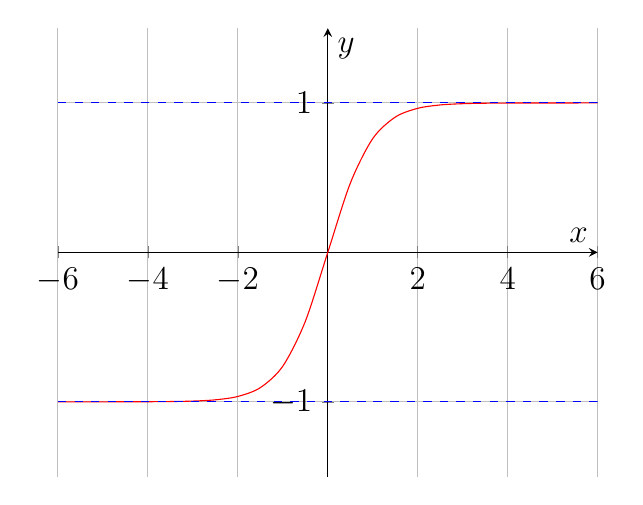
\begin{tikzpicture}
  \begin{axis}[domain=-6:6,ymin=-1.5,ymax=1.5, grid=both, font=\large, axis lines = middle, smooth, xlabel={$x$}, ylabel={$y$}]
    \addplot[draw=red] {(e^x - e^(-x)) / (e^x + e^(-x))};
    \addplot[dashed, draw=blue] {-1};
    \addplot[dashed, draw=blue] {1};
    \node at (axis cs:1,1.8) {$th(x) = \frac{e^x - e^{-x}}{e^x + e^{-x}}$};
  \end{axis}
\end{tikzpicture}
